\subsection{Построение прокси переменной для коррупции}

\begin{frame}
\frametitle{Построение прокси переменной для местной коррупции}
	\begin{itemize}
		\item Задача - оценить уровень коррупции в госзакупках на субрегиональном уровне
		\item Доступный показатель - индекс восприятия коррупции (CPI) - слишком субъективен
		\item Вместо него - корреляция между выводом денег в период выборов и распределением госзакупок
		 между фирмами в данном районе
		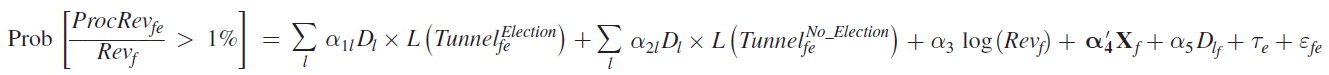
\includegraphics[scale=0.3]{images/kek1}
		\item Непрерывная переменная: t-статистика коэффициента $\alpha_1$
		\item Бинарная: 1, если $\alpha_1$ > 0 и значим на 10\%-ном уровне; 0 - иначе
	\end{itemize}
\end{frame}


\begin{frame}
\frametitle{Построение прокси переменной для местной коррупции}
	\begin{itemize}
		\item Плюсы в сравнении с CPI: 
		\begin{itemize}
			\item используются объективные данные
			\item доступен для всей районов
		\end{itemize} 
		\item Допущение при построении переменной: все доходы от бизнес деятельности фирмы получают не наличными, а банковскими платежами (иначе нет смысла выводить деньги, поскольку можно не регистрировать часть доходов и использовать эту часть для взяток)
		\item Предпосылка уместна, так как госконтракты получают в основном достаточно крупные фирмы, которые получают доходы не наличными 
	\end{itemize}
\end{frame}

\subsection{Проверка гипотезы}
\begin{frame}
\frametitle{Коррупция и эффективность тендеров}
	\begin{itemize}
		\item Гипотеза: в более коррумпированных регионах более эффективные фирмы используют взятки для обхода бюрократии, чтобы получить доступ к госзаказам
		\item Данные:
		\begin{itemize}
			\item 19113 фирм (крупнейшие)
			\item Районы с доступной информацией о коррупции
			\item Эффективность фирм: выручка на 1 сотрудника в 2003 году (из официальной отчетности фирм)
			\item Коррупция: построенная авторами прокси переменная
		\end{itemize}
	\end{itemize}
\end{frame}


\begin{frame}
\frametitle{Коррупция и эффективность тендеров: результаты модели}
	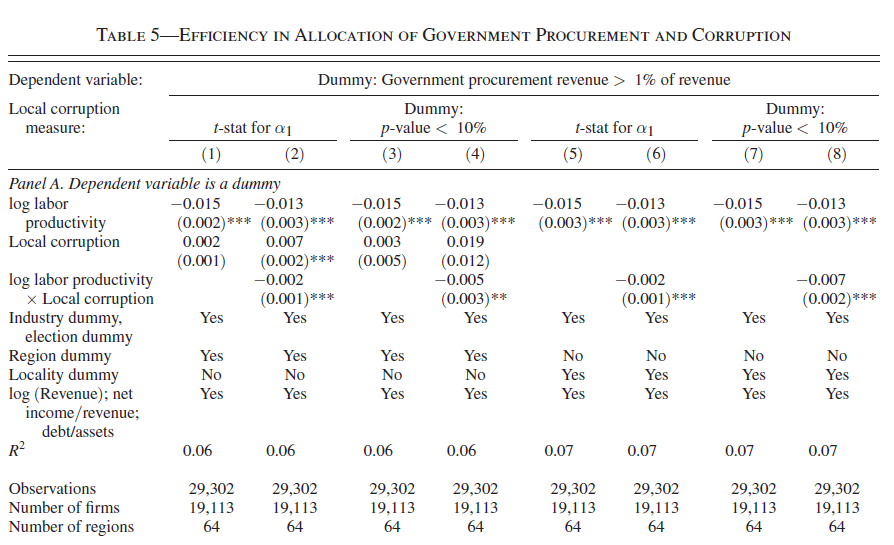
\includegraphics[scale=0.38]{images/kek2}
\end{frame}


\begin{frame}
\frametitle{Коррупция и эффективность тендеров: результаты модели}
	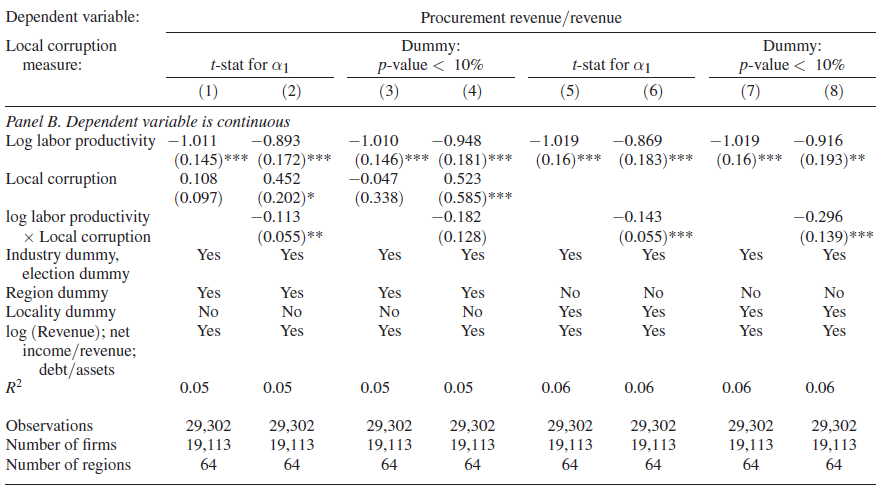
\includegraphics[scale=0.38]{images/kek3}
\end{frame}


\subsection{Выводы}
\begin{frame}
\frametitle{Коррупция и эффективность тендеров: выводы}
	\begin{itemize}
		\item Распределение госконтрактов неэффективно
		\\ИЛИ
		\item Госконтракты распределяются таким образом, чтобы поддерживать высокий уровень занятости (политика патронажа)
		\medskip\hrule\medskip
		\item В более коррупционных районах госзаказы получают менее производительные фирмы
		\item Полученные результаты устойчивы относительно разбиения выборки на коррумпированные и некоррумпированные районы
		\item Гипотеза о том, что взятки являются "смазкой" бюрократической системы не подтвердилась
	\end{itemize}
\end{frame}
